%!TEX root = ./main.tex
\chapter{Background}

The purpose of this chapter, is to cover some background material, giving the reader a foundation for the later chapters. A introduction to the kNN problem is given, and it's relation to All-kNN, and Q-kNN problem is discussed. In addition, relevant parallel programming principles, practices and tools are presented.

\section{The k-nearest neighbors search problem} % (fold)
\label{a_short_introduction_to_kNN_search_problem}

The k-nearest neighbors (kNN) search problem, is, the problem of locating the $k$ closest neighbors to a given query point, with $k$ being some positive natural number. This is intuitively a quite simple problem to grasp, and for most of our purposes, an intuitive understanding of the problem will be sufficient, but let us start by looking a bit closer at the properties of kNN search in general.

If we consider $p$ to be a point in d-dimensional space so that $p = [x_1, x_2,\dots, x_d]$. Given a set of size $m$, consisting of such points $S = [p_1, p_2,\dots, p_m]$, a additional query point $q$, also in d-dimensional space, and some distance metric $D = f(p, q)$, the kNN problem is to find k points in $S$, such that the sum of distances in relation to $q$ is minimized. We introduce the term reference points to be the set $S$, to differentiate it from the query points $Q$. 

It is worth to note that since we are not limited, either in the number of dimensions, or distance metric we choose, the kNN problem is applicable in many different situations. If we e.g.\ wanted to construct a system for finding beer with similar flavor to one beer we just tasted, we could build a database of different beers, categorized by flavor dimensions like bitterness, maltiness, sweetness, and so on. Then, to find beers similar in flavor to the one we just tasted, we would perform a kNN query on this database, using a suitable distance metric, and the beer we just tasted as our query point.

The general nature of the kNN problem makes it relevant in many research and industrial settings, from 3-d object rendering, content based image retrial, statistics and biology \citep[Introduction]{Garcia2010}.

When wanting to query point cloud data, one can make some simplifications to this general kNN problem. In our research we are only concerned with three spacial dimensions, and their Euclidean relations. 

This is not a universal way to simplify the kNN problem to point cloud data, and other dimension might be interesting to add for other applications. Other metrics commonly related to point cloud data, e.g.\ the color value of each point, could also be interesting to include. But for most applications, TSI application included, three dimensions, and an Euclidean distance metric is all we need. Throughout this text we will use the term kNN to refer to this simplification of the kNN problem.

When studying point clouds, it can be interesting to find the k-closest points to all points in the point cloud. In order to compute this, you would simply perform kNN queries, using all the points in the point cloud as query points. In order to refer to this variant of the kNN search problem, we will use the term All-kNN\@.

Another similar variant of the kNN problem, is application of the kNN algorithm to a set of query points of size q. In this version of the problem, you are not limited to the query point set being the points in the point cloud, it can be any set of three dimensional points. We will refer to this problem variant as Q-kNN, and note that All-kNN is a subproblem of Q-kNN\@.
% section a_short_introduction_to_kNN_search_problem (end)

\section{A short introduction to parallel programming principles} % (fold)
\label{sub:a_short_introduction_to_relevant_parallel_programming_principles}

Parallel programming is programming targeting parallel computing, where sections of the program is executed simultaneously on multiple cores, processors, machines, or other suitable environments. We use the term parallelization to mean transformation of computational instructions intended for sequential execution to simultaneous, or parallel, execution.

Parallelization can be introduced on several different levels in a computer. Bit-level parallelization, where bit level operations is parallelized within a processor as is the case for 64-bit, 32-bit, 16-bit, etc.\ processors, being a common low level form. In order to avoid confusion, this text is not concerned with such levels of parallelization, but will instead focus on higher level parallelization, related to developing and implementing algorithms in a regular programming language. We will also use the term parallel unit as a general term for a single computational unit in a theoretical parallel machine, with a unlimited number of parallel units.

It is easy to grasp that parallelization can speed up the execution of a program. Given a problem where we want to add one to every element in a list of numbers. In a sequential program we could go through the list of numbers, adding one to each element in each step. This would roughly take the time needed for adding one number to another, times the number of elements in the list. In out theoretical parallel machine, we can simply assign all the elements in the list to a different parallel unit and ask every unit to add one to it's assigned number. This would take much less time than the sequential algorithm, just the time needed to add a number, since all numbers in the list is added at the same time.

Adding one to the elements of a list is a trivial problem, and unfortunately not all problems can be parallelized as easy as this. Even simple problems can be hard to parallelize. Consider adding all the numbers together, instead of adding one to each number. This is a very similar problem, we still only has to add a number to all of the elements in the list. The problem is that we does not know what to add to a given element before all the previous elements has been added together. We could calculate the sub-sum of small subsections of the list in parallel, and then add the resulting sub-sums together in a sequential fashion, but then a part of our program does not execute in parallel. This exemplifies, that for many problems, we cannot entirely parallelize the execution, because some data has to be transfered between the threads. We need a way to let the parallel units communicate with each other.

Communication is often a large factor in limiting the performance that can be harnessed from parallelization. Communication can be the source of implied sequential execution, since the parallel units have to wait for data from another unit. It is also often inherently slow, and carries a high overhead due to low data transfer speeds between hardware components. The possibility of minimizing the amount of communication, is therefor a major factor in determining if a sequential algorithm can be successfully parallelized.

\subsection{Shared memory architecture} % (fold)
\label{sub:shared_memory_architecture}

In a parallel computer using shared memory architecture (SMA), the different parallel units all share a global shared memory. The parallel units usually are different processors, often located within the same physical chip like a multi-core CPU\@. 

This is the architecture used by most modern desktop computers. Different varieties exist, with separate processor cache for each processor core, shared cache or even a combination, with shared L2 cache and distributed L1 cache. From the point of view of this thesis, all these varieties would fall under the SMA classification.

Shared memory is easy to work with and understand, and communication between different parallel units can be facilitated quite easily, and relatively fast, by reading and writing the same memory. The drawback is that the programmer must ensure that the different parallel units does not try to access the same memory at the same time, or in the wrong order. SMA still works well for smaller parallel computer systems.
% subsection shared_memory_architecture (end)

\subsection{Distributed memory architecture} % (fold)
\label{sub:distributed_memory_architecture}

In a computer system using distributed memory architecture (DMA), each parallel unit contains both processor and memory. The processor can only access data from it's own local memory, and if data is needed from another parallel unit, it has to be transfered from that units local memory into the memory of the unit in need of the data. DMA computer systems usually scales better when using a high number of parallel units, compared to SMA systems, since one memory does not have to facilitate all parallel units. The drawback is that communication carries a higher overhead, since data has to be transferred between the different local memories of each unit.

Computer systems using a distributed memory architecture, often resemble many individual computers, working in parallel on the same problem, and communicating using specialized networking components.

This is the architecture favored in todays supercomputers. Many varieties exist, especially concerning the network layout between the different machines. Since each individual parallel unit in such systems usually can be considered to be an individual computer, each unit often has a internal shared memory architecture, like desktop computer. This makes the entire system capable of harnessing the strength of both SMA and DMA, but increases the complexity that the programmer has to handle. As we will discover later in the text, GPUs are organized using an architecture with this kind of hybrid architecture.
% subsection distributed_memory_architecture (end)

\subsection{Parallel speedup} % (fold)
\label{sub:parallel_speedup}

Parallel speedup, or just speedup as it is often called, is a measure of how much faster a parallel algorithm is compared to it's sequential counterpart.

Let $T_s$ be the execution time of the sequential algorithm, and $T_p$ be the execution time of the parallel algorithm on a system with $p$ parallel units. The speedup $S_p$ is then defined as $S_p = T_s / T_p$.

In the ideal situation, the relation between the speedup and the number of parallel units will be linear. Due to overhead related to possible communication, and the use of a more complex framework for the parallel code, this is usually not possible to achieve. We therefore have the parallel efficiency metric $E_p = S_p / p$, which describes how much is lost to such factors.

Speedup and efficiency can be a good measure of how well the algorithm is parallelized, but it can not necessarily be used to determine if one parallel algorithm is faster than another. Parallelizing many inefficient brute-force algorithms can be done with excellent speedup and efficiency, but the resulting algorithm will often be considerably slower than the parallel version of a better sequential algorithm, or even just a better sequential algorithm. Parallelizing bad code will result in just as bad code, and thorough study of efficient algorithms should always be carried out before attempting any parallelization.
% subsection parallel_speedup (end)

\subsection{The APOD design cycle} % (fold)
\label{sub:the_apod_design_cycle}

In order to work efficiently with parallelization problems, many programmers adopt a work-flow similar to the APOD design cycle\citep[Preface]{cuda_c_best_practices_guide}. The cycle consists of four steps:

\begin{enumerate}
    \item \textbf{Assess:} Locate the parts of the code which take up most of the run-time. Re-writing an entire application for parallel execution is usually very hard and time consuming, if it is even possible. The best results for the user might be to just parallelize the one algorithm that is taking a long time to execute. Parallelization might not even be the answer, a faster sequential algorithm could also be a solution or part of the solution.

    \item \textbf{Parallelize:} Investigate if any pre-written library of parallel functions could be used as part of, or the entire solution. Try to pinpoint which part of the code that can execute in parallel, and which part is dependent on communication. If the code is inherently dependent on communication, sequential alternatives, more suitable for parallelization, might be researched. Just not be tempted to use a inefficient algorithm because it is easy to parallelize.

    \item \textbf{Optimize:} Dependent on the parallel computer system, programming language, and other tools you are using, a number of conventional optimization strategies might be applied. This should not be forgotten when writing parallel code. On a CUDA GPU you will often want to check that you are using the optimal type of memory for different tasks, minimize the divergence in the code and try to optimize the use of arithmetic operations. 

    \item \textbf{Deploy:} Run your application on real hardware, test thoroughly, and compare the results to the original. Did the parallelization actually increase the performance of the application? Deploy the code to potential users. They will benefit from the increased performance, and you will get feedback if any bugs exist.
\end{enumerate}
% section a_short_introduction_to_relevant_parallel_programming_principles (end)

\section{A short introduction to GPU programming and CUDA} % (fold)
\label{sub:a_short_introduction_to_gpu_programming_and_cuda}

Moore's law has been a gift to all programmers the past 50 years. The law predicts that performance of integrated circuits would double every two years, and it has become the de facto standard for computer processing capabilities since it was first stated. However, since the so called Power Wall in 2002, the world of computer hardware performance has been changing. In order to keep up with Moore's law, the hardware vendors have been mowing from single core processors, where all computation is performed by one fast processor core, to processors with multiple cores, working in parallel. As a result, many programs and algorithms has to be rewritten, in order to benefit from this new hardware architecture.

In recent years, many tools for working with parallel programming, has been developed. Frameworks and libraries like OpenMP, CUDA, MPI and OpenCl being some of the more notable examples. These tool support various types of parallel hardware architecture.

OpenMP supports parallelization, targeting shared memory architecture. It is an implementation of multi threading, whereby a master thread divide the workload to different forked slave threads.

The Message Passing Interface (MPI), is a library specification for message passing, often used for parallel programming, targeting distributed memory architecture. It is maintained and promoted by a committee, consisting of a wide selection of academics, hardware and software vendors.

In the consumer marked, GPUs represent hardware with a high number of parallel units compared to the price. The NVIDIA GeForce GTX 480 GPU is e.g able to execute 23,040 threads in parallel \citep{karras2012}. The reason GPUs can have such a massive amount of parallel units at this price point, compared to traditional hardware like a CPU, is that each parallel thread is very lightweight. Individually, each thread has relatively low performance, but together they can achieve an extremely high instruction throughput. This makes targeting the GPU, a good solution for high performance parallel computing on a desktop computer.
% section a_short_introduction_to_gpu_programming_and_cuda (end)

\subsection{General-purpose computing on graphics processing units} % (fold)
\label{ssub:general_purpose_computing_on_graphics_processing_units}

GPGPU is the utilization of a GPU in applications to perform heavy computations, normally handled by the CPU\@. This is most efficiently accomplished by using GPGPU specific programming tools. Two widely tools approaches are the Compute Unified Device Architecture (CUDA) and the Open Compute Language (OpenCL).

OpenCl is a low-level framework for heterogeneous computing for both CPU and GPU's. It includes a programming language, based on C99, for writing kernels. Kernels are methods that executes on the GPU\@. It also includes an API that are used to define and control the platform.

In contrast to the open OpenCL, the dominant proprietary framework, CUDA\@, is only designed for GPU programming. It is, as OpenCL, based on a programming language and a programming interface. Science CUDA is created by the vendor, it is developed in close proximity with the hardware.

For a deep and thoroughly survey of GPGPU programming, techniques and applications take a look at John D. Owens article from 2007 \citep{Owens:2007:ASO}.
% subsection general_purpose_computing_on_graphics_processing_units (end)

\subsection{NVIDIA GPU architecture} % (fold)
\label{ssub:nvidia_gpu_architecture}

A CPU is usually optimized for low memory latency. This enables the CPU to quickly fetch data and instructions from memory. For a chip to achieve low latency, it needs to have a large amount of cache available. This makes it hard to physically fit a very many cores on a single chip.

The GPU is optimized for high throughput. Throughput is a metric of how fast a processor is able to process data, and this is desirable when processing graphics, where a data has to be updated fast, in order to redraw the screen. To achieve high throughout, a large number of cores, or ALUs, are needed. GPUs is therefore usually organized with a small control unit and cache, but a large number of cores.

A NVIDIA GPU is build around a scalable array of multi-threaded Streaming Multiprocessors (SMs). A multiprocessor are designed to execute hundreds of threads concurrently. It is organized according to an architecture called Single-Instruction, Multiple-Thread (SIMT), where each SMs creates, manages, schedules and executes parallel threads in groups of 32, called a warp. Threads composing a warp starts at the same program address, but they have their own register state and instruction address, and is therefore free to branch and execute independently \citep{cuda_programming_guide}.

\begin{figure}[ht!]
    \centering
    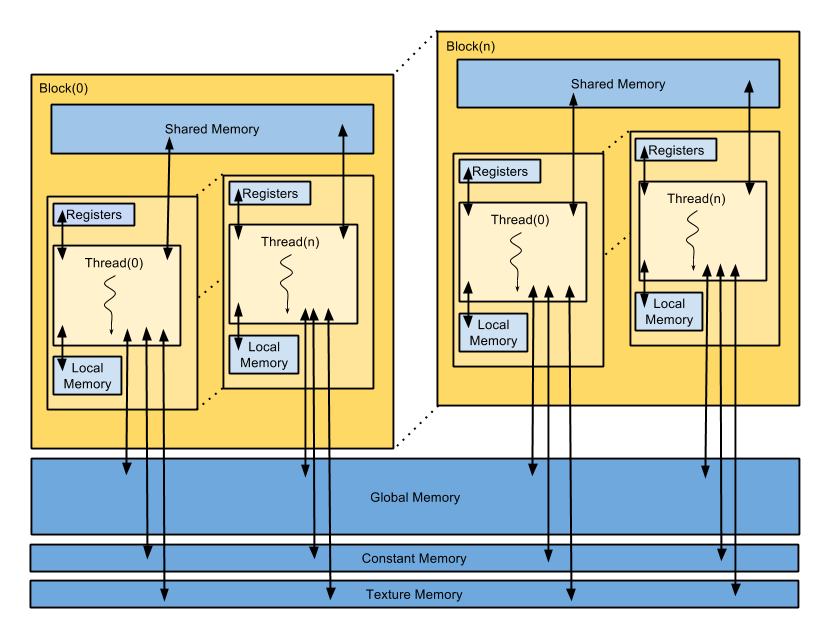
\includegraphics[width=100mm]{../gfx/memory_hierarchy.png}
    \caption{A visualization of the memory hierarchy in CUDA.}
    \label{fig:memory_hierachy}
\end{figure}

An other impotent part of the GPU architecture is the memory hierarchy, see Figure~\ref{fig:memory_hierachy}. Global memory is bottom-most part of this hierarchy and is analogous to RAM on the CPU\@. The global memory can be used to transfer memory to and from the host CPU\@. Each SM contains a fast L1 on-chip memory, which is divided into a shared memory and a cache. The fast shared memory is shared across each thread in a block, and resembles the shared memory found on the CPU\@. The threads also have their own 32-bit registers. Other types of memory also exist. Constant memory and texture memory are read-only, and therefore highly cacheable. Compared to the CPU, the peak floating-point capability and memory bandwidth of the GPU, is an order of magnitude slower \citep{Liangcu}.

As better hardware is developed by NVIDIA, some properties change. These changes are clustered into versions, called compute capabilities. All NVIDIA devices are backward compatible, so a device with compute capability of $3.x$ also have all properties that is found in compute capability $1.x$.  
% subsection nvidia_gpu_architecture (end)

\subsection{CUDA programming model} % (fold)
\label{ssub:cuda_programming_model}

The CUDA programming model is designed to make the heterogeneous GPU/CPU programming easier. The GPU works as a computation accelerator for the CPU, and the programming model should therefore be a bridge between the two. CUDA have created this bridge based on a runtime library, compiler and C language extensions. The C language extensions, enables the programmer to create and launch methods on the GPU, through the runtime library. These methods are called kernels.

A CUDA program, is based on a data-parallel behavior, where threads are executed in parallel. The execution of a kernel, is organized as a grid of blocks consisting of threads, see Figure~\ref{fig:thread_block}. When a kernel grid is launched on the host CPU, blocks of the grid is enumerated and distributed among the SMs. The blocks then executes concurrently on each SM\@. Only threads in a block can communicate with each other. This is done by creating synchronization walls. Communicate can also be facilitated through the fast shared memory, located on the individual SMs\@. Each block and thread have their own id, which often is used to determines what portion of data the thread should process.

\begin{figure}[ht!]
\centering
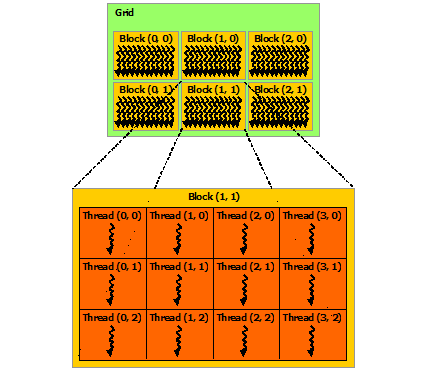
\includegraphics[width=75mm]{../gfx/blocks_and_threads.png}
\caption{The relationship between threads and blocks in a grid~\cite{cuda_programming_guide}.}
\label{fig:thread_block}
\end{figure}
% subsection cuda_programming_model (end)
% section a_short_introduction_to_gpu_programming_and_cuda (end)

\cleardoublepage
